
%%%%%%%%%%%%%%%%%%%%%%%%%%%%%
% Standard header for working papers
%
% WPHeader.tex
%
%%%%%%%%%%%%%%%%%%%%%%%%%%%%%

\documentclass[11pt]{article}



%%%%%%%%%%%%%%%%%%%%%%%%%%
%% TEMPLATES
%%%%%%%%%%%%%%%%%%%%%%%%%%


% Simple Tabular

%\begin{tabular}{ |c|c|c| } 
% \hline
% cell1 & cell2 & cell3 \\ 
% cell4 & cell5 & cell6 \\ 
% cell7 & cell8 & cell9 \\ 
% \hline
%\end{tabular}





%%%%%%%%%%%%%%%%%%%%%%%%%%
%% Packages
%%%%%%%%%%%%%%%%%%%%%%%%%%



% encoding 
\usepackage[utf8]{inputenc}
\usepackage[T1]{fontenc}


% general packages without options
\usepackage{amsmath,amssymb,amsthm,bbm}

% graphics
\usepackage{graphicx,transparent,eso-pic}

% text formatting
\usepackage[document]{ragged2e}
\usepackage{pagecolor,color}
%\usepackage{ulem}
\usepackage{soul}


% conditions
\usepackage{ifthen}


\usepackage{booktabs}
\usepackage{threeparttable}



%%%%%%%%%%%%%%%%%%%%%%%%%%
%% Maths environment
%%%%%%%%%%%%%%%%%%%%%%%%%%

%\newtheorem{theorem}{Theorem}[section]
%\newtheorem{lemma}[theorem]{Lemma}
%\newtheorem{proposition}[theorem]{Proposition}
%\newtheorem{corollary}[theorem]{Corollary}

%\newenvironment{proof}[1][Proof]{\begin{trivlist}
%\item[\hskip \labelsep {\bfseries #1}]}{\end{trivlist}}
%\newenvironment{definition}[1][Definition]{\begin{trivlist}
%\item[\hskip \labelsep {\bfseries #1}]}{\end{trivlist}}
%\newenvironment{example}[1][Example]{\begin{trivlist}
%\item[\hskip \labelsep {\bfseries #1}]}{\end{trivlist}}
%\newenvironment{remark}[1][Remark]{\begin{trivlist}
%\item[\hskip \labelsep {\bfseries #1}]}{\end{trivlist}}

%\newcommand{\qed}{\nobreak \ifvmode \relax \else
%      \ifdim\lastskip<1.5em \hskip-\lastskip
%      \hskip1.5em plus0em minus0.5em \fi \nobreak
%      \vrule height0.75em width0.5em depth0.25em\fi}


%% Commands

\newcommand{\noun}[1]{\textsc{#1}}


%% Math

% Operators
\DeclareMathOperator{\Cov}{Cov}
\DeclareMathOperator{\Var}{Var}
\DeclareMathOperator{\E}{\mathbb{E}}
\DeclareMathOperator{\Proba}{\mathbb{P}}

\newcommand{\Covb}[2]{\ensuremath{\Cov\!\left[#1,#2\right]}}
\newcommand{\Eb}[1]{\ensuremath{\E\!\left[#1\right]}}
\newcommand{\Pb}[1]{\ensuremath{\Proba\!\left[#1\right]}}
\newcommand{\Varb}[1]{\ensuremath{\Var\!\left[#1\right]}}

% norm
\newcommand{\norm}[1]{\left\lVert #1 \right\rVert}



% argmin
\DeclareMathOperator*{\argmin}{\arg\!\min}


% amsthm environments
\newtheorem{definition}{Definition}
\newtheorem{proposition}{Proposition}
\newtheorem{assumption}{Assumption}

%% graphics

% renew graphics command for relative path providment only ?
%\renewcommand{\includegraphics[]{}}








% geometry
\usepackage[margin=2cm]{geometry}

% layout : use fancyhdr package
\usepackage{fancyhdr}
\pagestyle{fancy}

\makeatletter

\renewcommand{\headrulewidth}{0.4pt}
\renewcommand{\footrulewidth}{0.4pt}
\fancyhead[RO,RE]{\textit{Working Paper}}
\fancyhead[LO,LE]{CASA/ISC-PIF}
\fancyfoot[RO,RE] {\thepage}
\fancyfoot[LO,LE] {\noun{J. Raimbault}}
\fancyfoot[CO,CE] {}

\makeatother


%%%%%%%%%%%%%%%%%%%%%
%% Begin doc
%%%%%%%%%%%%%%%%%%%%%

\begin{document}






\begin{document}


\title{Coupling microsimulation models with land-use transport models}

%\author{}
\date{}

\maketitle

\justify


\begin{abstract}
	We describe here preliminary investigations towards the coupling of a land-use transport interaction model with a population microsimulation model, at the scale of a country. We situate the approach within the scientific landscape in terms of citation networks around works dealing with microsimulation. We then compare the characteristics of the two models and build on their complementarity to suggest research directions towards this coupling. 
\end{abstract}




%%%%%%%%%%%%
\section{Introduction}


A strong need of multi-scalar models to be applied to sustainable policy making is already shaping the construction of the next generation of territorial models \cite{Rozenblat2018}. Indeed, the coupling of complementary modeling approaches to the same systems is coined by \cite{banos2013pour} as an essential step forward in social simulation to be able to better tackle the complexity of such systems. The modeling activity must furthermore be highly integrated with other knowledge domains \cite{raimbault2017applied}, in particular empirical and theoretical approaches, to foster the production of applicable complex knowledge.

The QUANT land-use transport interaction model \cite{batty2019generalized} responds to this constraints as it integrates fine data for population, employments and transportation at the scale of all UK, while keeping a simple structure for the processes implemented. Integrating it with a complementary model, possibly at an other scale, would open new possibilities for the design of territorial policies.

In particular, population structure, demographic processes and dynamic aspects are not taken into account in the QUANT model, making microsimulation models \cite{birkin2011spatial} good candidates to be coupled with this model. The purpose of the type of microsimulation models we consider is to provide estimates of spatio-demographic trajectories of territories with a high precision, having an interest in themselves for projections, but also for local policies taking into account spatial heterogeneity and a variety of social processes which can be coupled with microsimulation (economics, crime, retail, health, environmental issues, etc.). The MOSES model embeds various heterogenous data and is able to simulate demographic trajectories at the Ward level on a 30 years time span \cite{townend2009moses,Wu2013} (this model is distinct from a much older Moses microsimulation model focused on economic processes \cite{eliasson1989moses}). A user interface and the connexion to computation infrastructure allow its use for real decision making problems \cite{birkin2009moses}. It has been applied for example for the study of the spatial distribution of crime by coupling it with an agent-based model \cite{malleson2012analysis}. We will develop here potential directions to couple the QUANT model with the MOSES model (or more precisely its successor, called SPENCER).

The literature is rather sparse on studies coupling spatial interaction models with microsimulation models. Examples include configurations where the spatial and demographic structure of population plays a role in its interaction with the object of study, such as retail \cite{Nakaya2007}, in spatial epidemiology \cite{morrissey2010examining}, or for socio-spatial simulations of a particular population \cite{wu2008spatial}. Beside possible policy applications, our approach can therefore also provide methodological contributions.





%%%%%%%%%%%%
\section{Scientific landscape}

For a better grasp of the issues at stake in the approach taken, we propose to map the scientific landscape around works in microsimulation. We apply a part of the method introduced by \cite{raimbault2017exploration}, namely backward citation network reconstruction and mapping, using the open source tools provided. The method to construct the citation network starts from an initial corpus, and retrieves citing references for each paper in the corpus, recursively up to a specified depth. Citation data is crawled from google scholar and results are conditional to this data source (which has a good coverage in comparison to the WoS or Scopus, but includes grey literature and preprints).

We construct the initial corpus with the 200 first responses to the request ``\texttt{microsimulation}'' and construct the citation network at depth 2 from these 200 references. We obtain a network with $\left|V\right|=146774$ nodes and $\left|E\right|=210341$ links, and an average in-degree of 1.43 (3.01 conditionally to have at least one citation). A Louvain community detection on the undirected network yields a directed modularity of 0.69, suggesting strong disciplinary patterns within the network.  

It is interesting to remark that the first level (initial corpus) is highly integrated in terms of citations, since it exhibits an average in-degree of 6.46 on the giant component (181 out of 200 references), as shown in Fig.~\ref{fig:citnwdepth0}. The communities obtained already suggest disciplinary and thematic patterns: a large community (purple) includes the SimBritain model \cite{ballas2005simbritain}, issues about validation and synthetic populations, and may be interpreted as a methodological community; an other large community (green) deals with policy application of microsimulation models; and an other one with inequalities (blue); two smaller communities are focused on health applications of microsimulation (dark green) and the link with agent-based models (red), whereas the smallest community is difficult to classify and includes the Sverige model \cite{holm2002sverige}. The papers associated to the model we will study are distributed in the policy community \cite{wu2012moses}, the methodological community \cite{townend2009moses} and the unclassified community \cite{rees2017moses}.

When studying the network at depth 1 (Fig.~\ref{fig:citnwdepth1}), a map of disciplines using microsimulation begin to emerge, and communities are at a lower granularity. Modularity is much higher (0.70). The proper microsimulation papers are split in a large community (blue) and two smaller ones (red and turquoise). We then observe two highly clustered communities corresponding to inequalities (green) and spatial statistics (purple). A community (orange) deals with the links with agent-based modeling. Finally, a community (in yellow) situated at the interface of ABM, microsimulation and spatial statistics deals with transportation and LUTI models, what is of particular interest for our positioning since it confirms the disciplinary relevance of coupling the two approaches and furthermore highlights issues which will be of first importance (the relation to ABMs for example).

At depth 2, the network shown in Fig.~\ref{fig:citnwdepth2} describes the much broader scientific environment of microsimulation models. We still obtain a highly clustered community around inequalities, whereas health geography and LUTI are integrated with spatial statistics and two other communities dealing with two other approaches to inequalities. An other isolated and clustered community focuses on epidemiology. The broad microsimulation clusters acts as a backbone of the network, having roughly a similar proximity with the different domains (which is due to the construction process of the network), at the exception of a high integration with geosimulation and Luti models. This higher integration confirms the relevance of the approach proposed.

Sensitivity to the initial corpus, by changing the number of initial references (and grasping smaller fields of application e.g.) or by starting with a list of specified papers, remains to be checked. Also some parts of literature at the interface of agent-based modeling and microsimulation, which terminology is closer to ABM (e.g. the MATSIM model in the case of transportation), may have been missed here. A more systematic review as done in \cite{raimbault2018caracterisation} in the case of models of interactions between transportation and territories, combining a broader initial semantic search and a corpus based on a preliminary literature review validated by expert knowledge, should provide a more exhaustive overview of the scientific landscape.


%%%%%%%%%%%%
\begin{figure}
  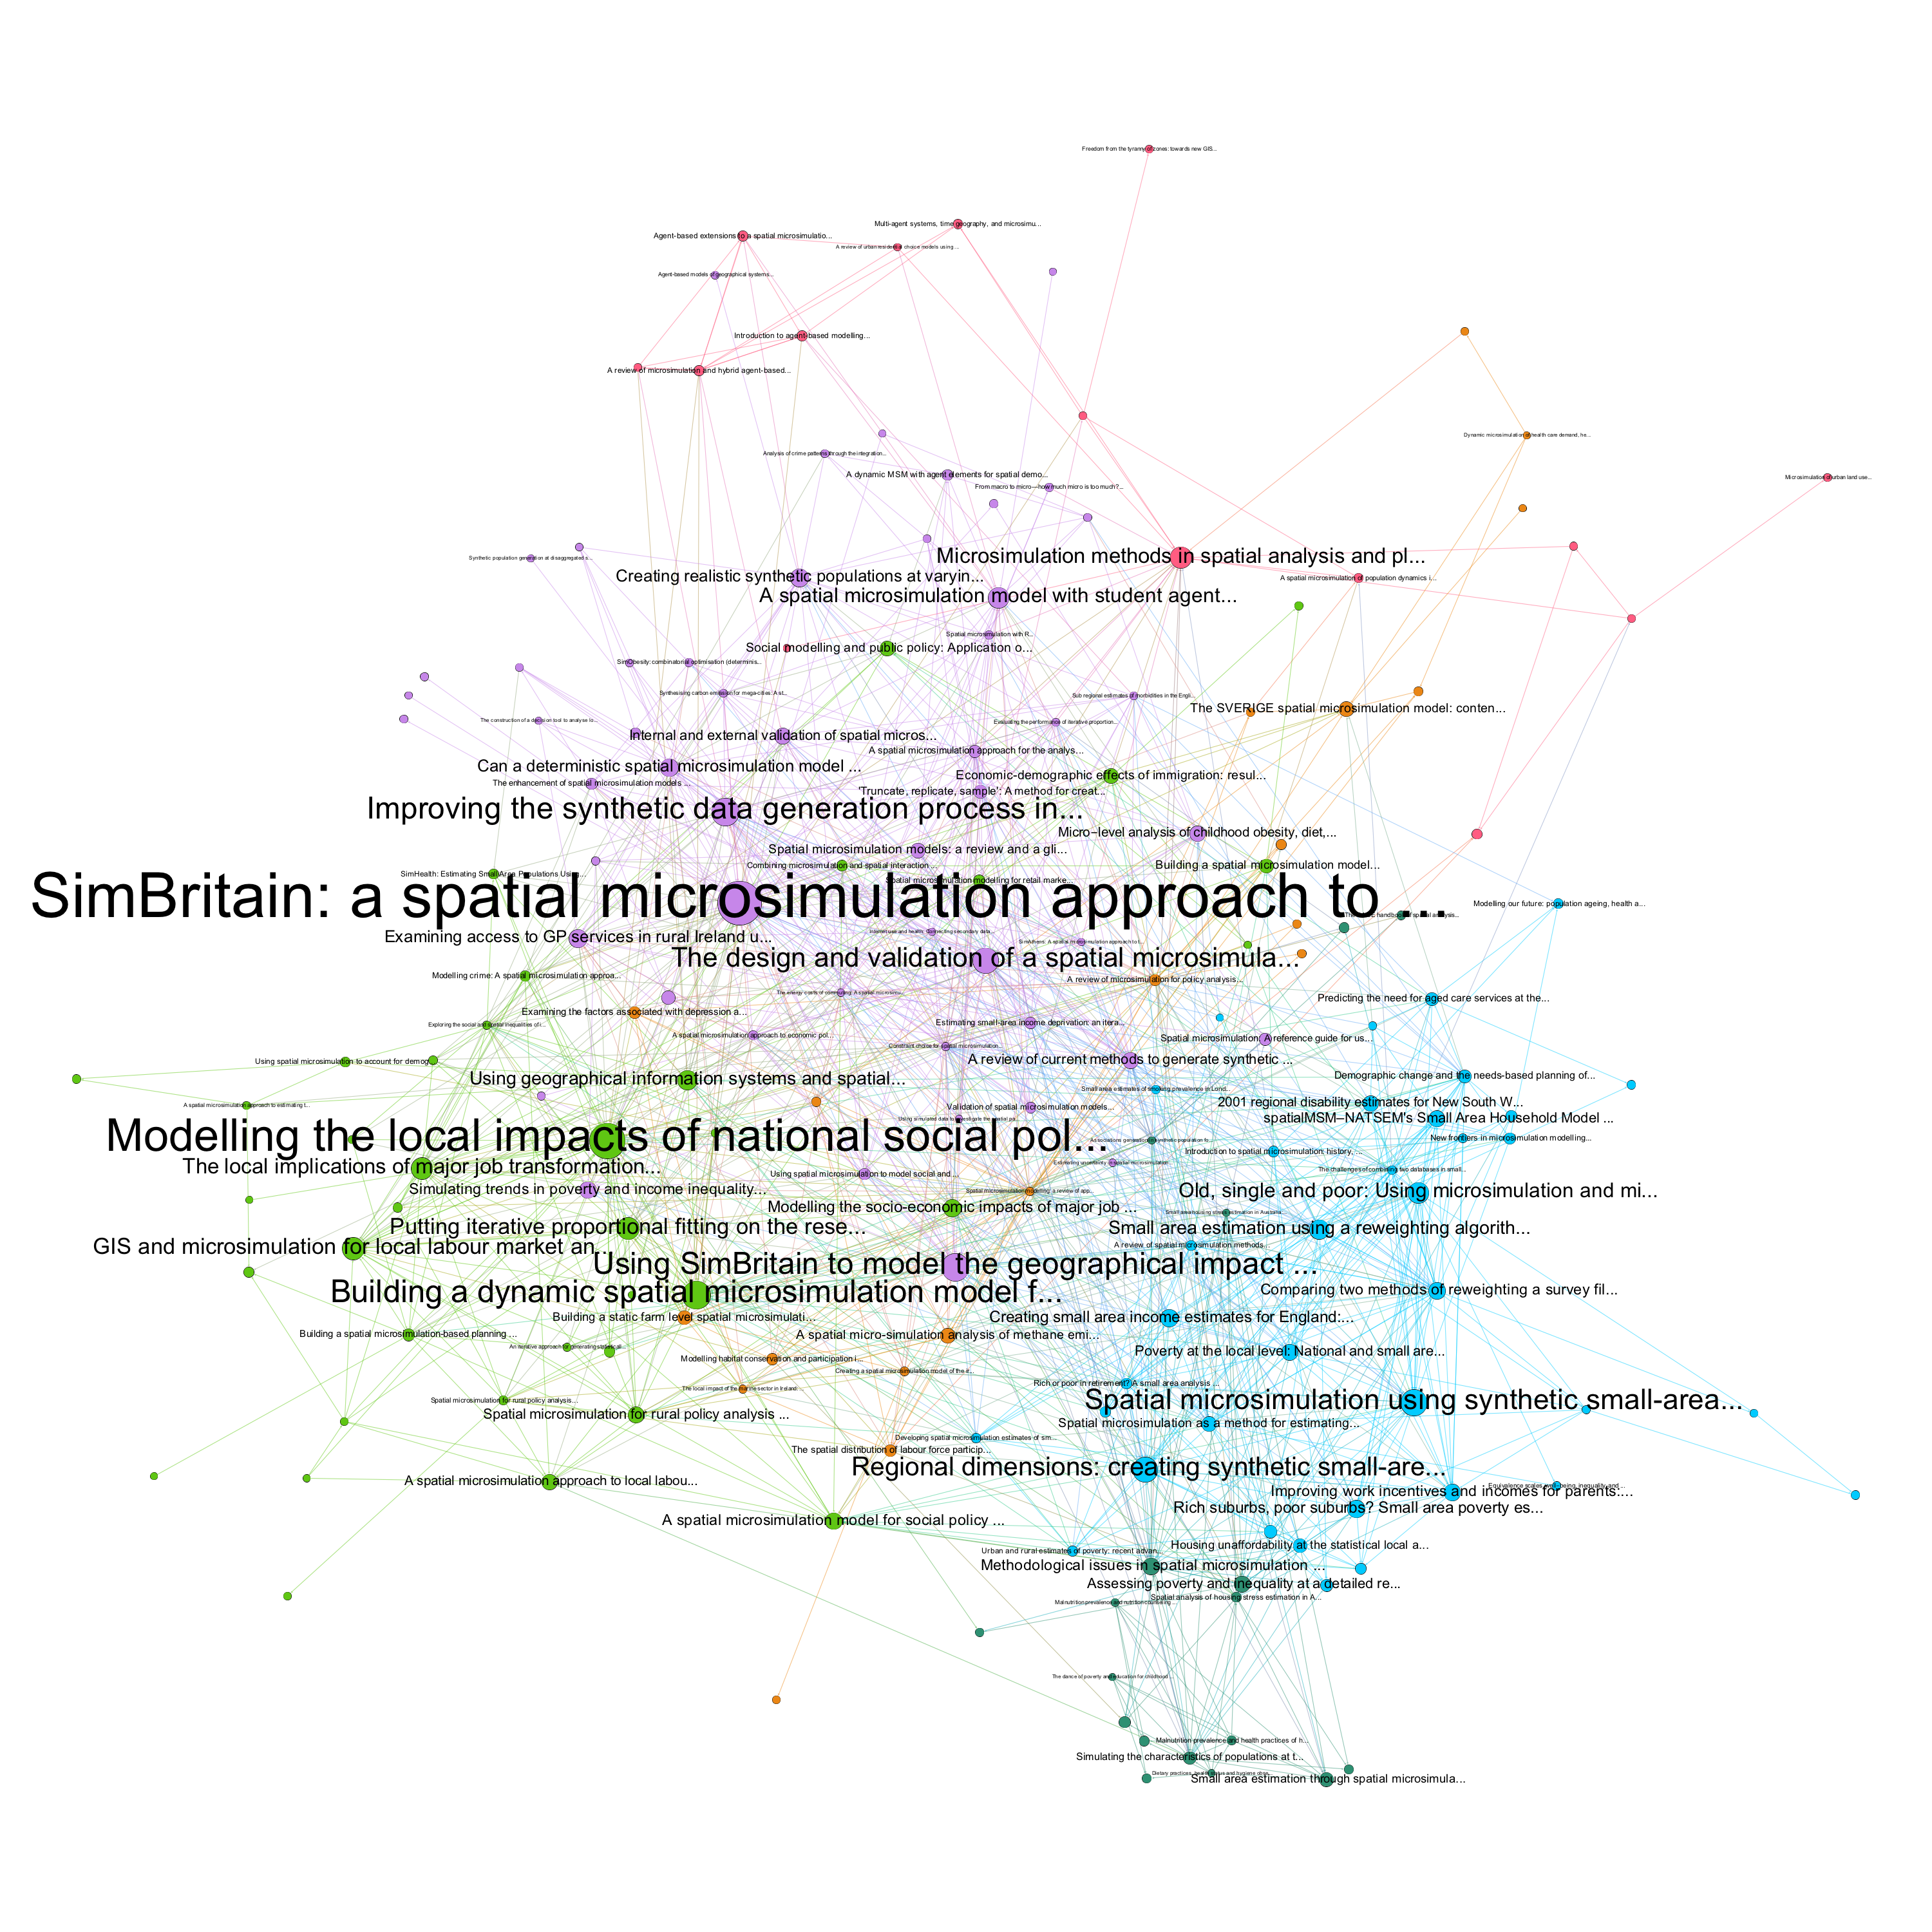
\includegraphics[width=\linewidth]{figures/microsim_depth0.png}
  \caption{Giant component of the citation network core at depth 0, i.e. 181 references out of the initial corpus with 200 references and the citation links between these. Average in-degree is 6.46 and Louvain modularity is 0.32.}
  \label{fig:citnwdepth0}
\end{figure}
%%%%%%%%%%%%


%%%%%%%%%%%%
\begin{figure}
  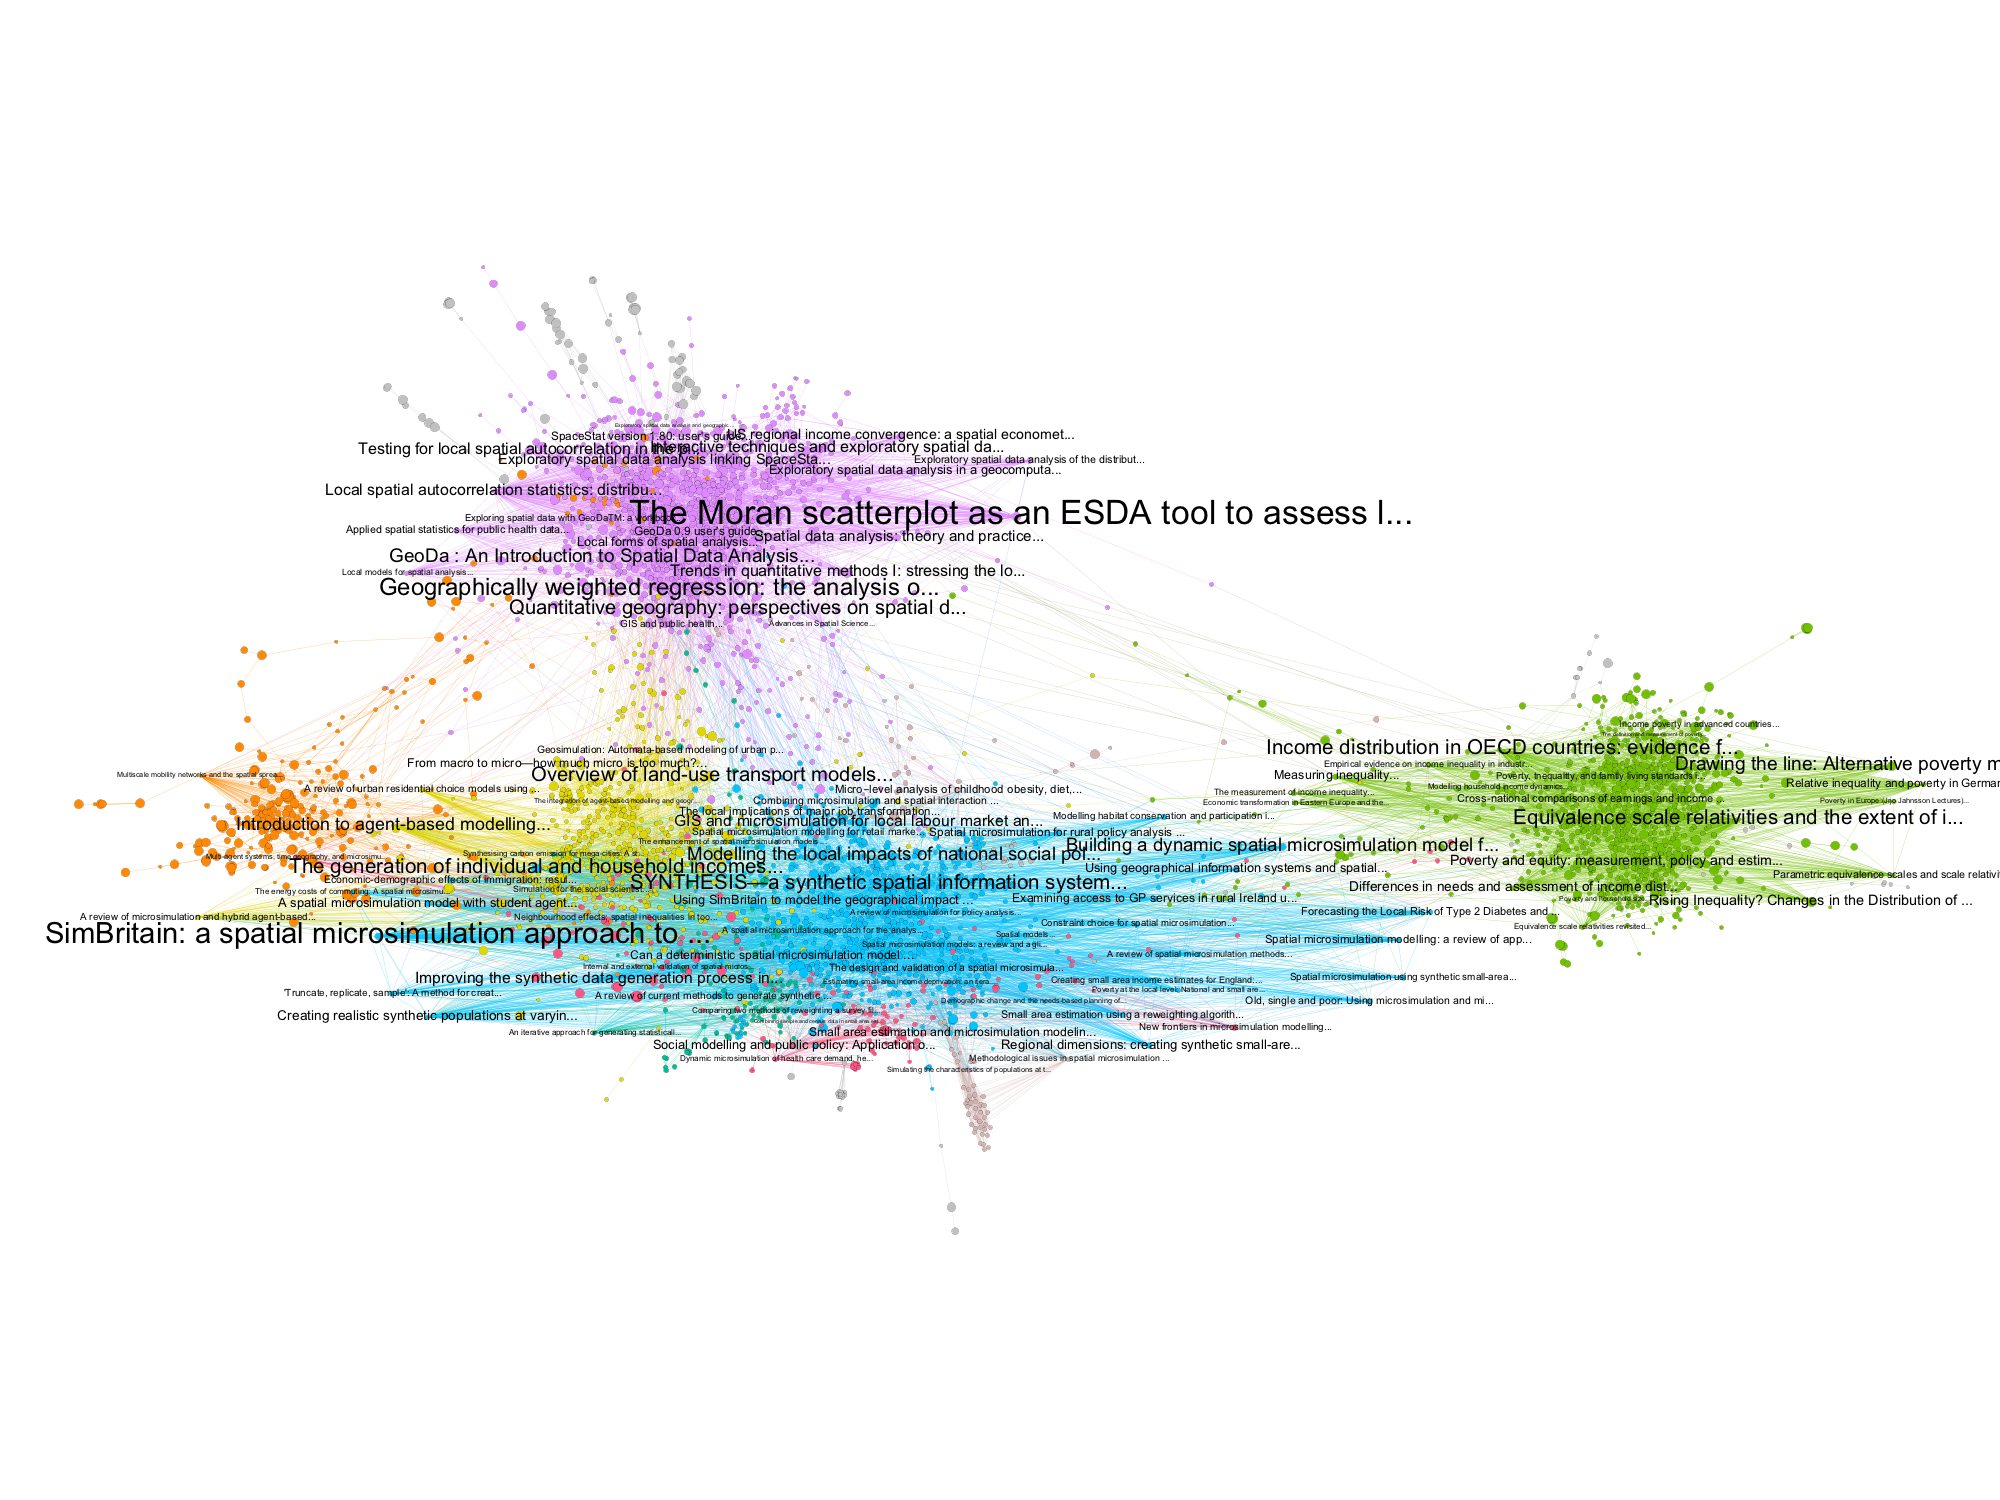
\includegraphics[width=\linewidth]{figures/microsim_depth1.png}
  \caption{Citation network core at depth 1. The core is constructed by removing all nodes having no citation, yielding a network of size $\left|V\right|=4846$ nodes and $\left|E\right|=15590$ links, average in-degree of 3.22 and modularity 0.70.}
  \label{fig:citnwdepth1}
\end{figure}
%%%%%%%%%%%%

%%%%%%%%%%%%
\begin{figure}
  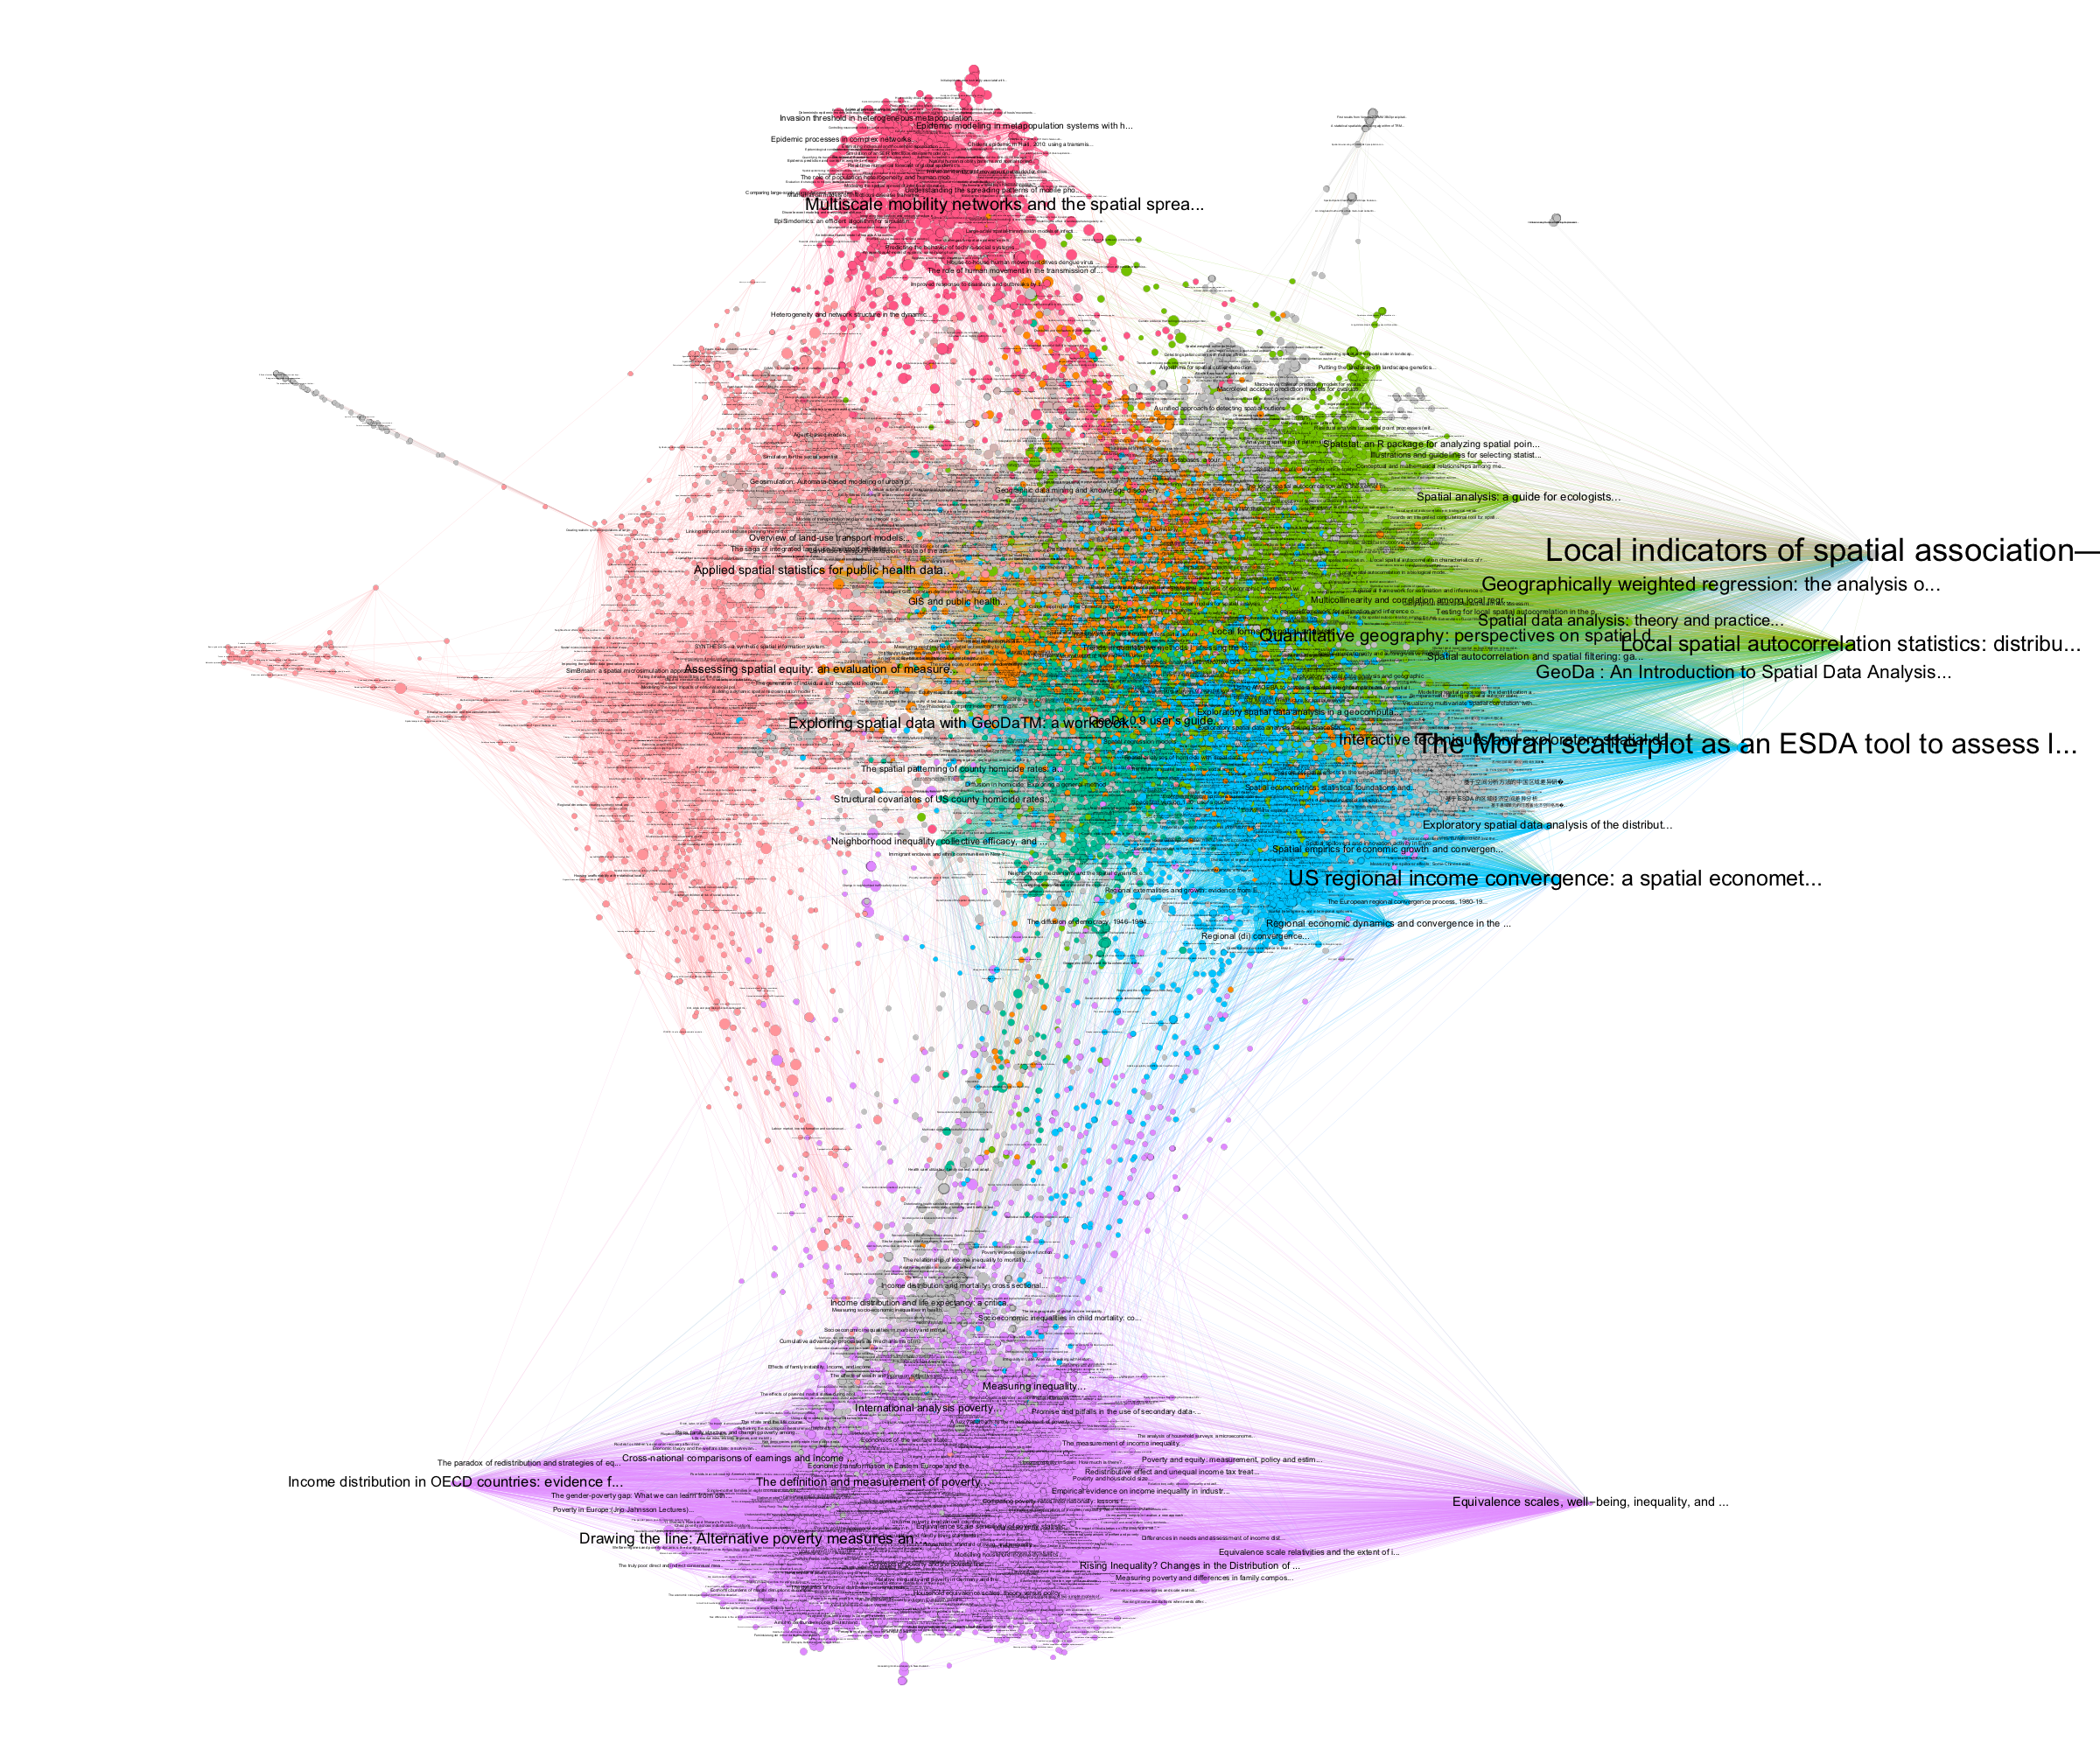
\includegraphics[width=\linewidth]{figures/microsim_depth2_corehigher.png}
  \caption{Citation network core at depth 2. For visibility purposes, we show here a ``higher order'' core, obtained by iteratively removing nodes of degree one until having only nodes with at least degree two. We have $\left|V\right|=31294$ and $\left|E\right|=94861$, an average in-degree of 3.03 and a modularity of 0.68.}
  \label{fig:citnwdepth2}
\end{figure}
%%%%%%%%%%%%




%%%%%%%%%%%%
\section{Complementarity of QUANT and MOSES}


We give in Table~\ref{tab:comparison} a rough comparison of QUANT and MOSES models main properties. This highlights the advantages of each and how they can complement each other. First of all, spatial and temporal scales, and spatial resolution, are reasonably comparable, implying that a coupling of these model should naturally be at the same level (although agent granularity is naturally different, the models are for this reason not exactly at the same level in terms of agents). The advantage should then be in the coupling of processes, by taking into account complementary aspects of the urban system that each model emphasizes. Indeed, when surveying processes included among the different components of the urban system, we observe that transportation and economic processes are not simulated in MOSES whereas they are part of the core of QUANT. On the contrary, demographic evolution is not simulated in QUANT but highly precise in MOSES. Finally, the movement of population in space is included in both but with different paradigms, since the microsimulation model uses migration probabilities estimated directly from real migration data whereas the Luti model distributes population according to accessibility patterns. The gordian knot of coupling will for this reason be on spatial population processes, as other aspects can be included without conflicting with the representation in the other model.



%%%%%%%%%%%%
\begin{table}
\begin{threeparttable}
	\caption{Main characteristics of QUANT and MOSES models.}\label{tab:comparison}
	\centering
	\begin{tabular}{|c|p{6cm}|p{6cm}|}
	\toprule
	& QUANT & MOSES \\
	\midrule
Time scale & 10 years $^{\ast 1}$ & 30 years \\
Spatial scale & UK & UK \\
Spatial resolution & Ward & Ward \\
Agent granularity & Aggregated counts & Person level \\
Static/Dynamic & Equilibrium (static) & Dynamic $^{\ast 2}$ \\
Randomness & Deterministic & Monte-Carlo simulations \\
Process: Transportation & 3 modes $^{\ast 3}$ & NA \\
Process: Economic activities & Accessibility-based relocations & NA \\
Process: Demographics & NA & Data-driven $^{\ast 4}$ \\
Process: Migration flows & Accessibility-based relocations & Data-driven \\
\bottomrule
	\end{tabular}
	\begin{tablenotes}
      \small
      \item $^{\ast 1}$ stylized time scale of metropolitan relocations \cite{wegener2004land}
      \item $^{\ast 2}$ model structure is however stationary - this is an important issue for a possible application to 2070
      \item $^{\ast 3}$ discrete choice for transportation mode is not implemented in QUANT \textbf{(?)} 
      \item $^{\ast 4}$ probabilities of basic demographic events (ageing, mortality, fertility, household formation, health, migration) are computed from data
    \end{tablenotes}
	\end{threeparttable}
\end{table}
%%%%%%%%%%%%



Possible coupling scenarios, with associated questions and potential outcomes, can be proposed:
\begin{itemize}
	\item Weak coupling Luti $\rightarrow$ microsimulation: using sequentially outputs of Quant as inputs of Moses. For example, evaluating a new transportation scenario will provide predictions for new populations, employments and commuting flows. Distributing the synthetic population and its movements conditionally to this new distribution (respecting reasonably some statistical properties of the original data, what may pose difficult synthetic data generation problems), and running the microsimulation model with this new parametrization, could provide micro-based measures of the impact of the new transportation line (e.g. exposure to pollution, access to health facilities, segregation, etc.). In that case, it does not seem to make much sense to use the aggregated prediction of the microsimulation model, since the uncertainty on input data will be high as a output of the upstream model (``\textit{garbage in-garbage out}''), and the coupled model has a prospective and scenario-testing function.
	\item Weak coupling Microsimulation $\rightarrow$ Luti: the other way around, population projections obtained with microsimulation, which should be more precise than relocations by Quant (assuming that the system remains stationary and that exogenous effects are reasonably included), can be used as an input of the Quant model, in order to apply it in future times when for example planning long term infrastructure projects. More accurate future populations will provide more accurate generalized accessibility projections given or not some modification of the transportation network. The question answered and model function would also be territorial prospective. %(\textit{Open question : how do model functions in the sense of the typology of \cite{varenne2017theories} evolve during model coupling, do some typical patterns exist or is it case/scale specific ? Given a ``strength'' of models (a partial order on a subset of models given some objectives), are there patterns on the strength of the coupled model ?})
	\item Both previous proposition make sense assuming large approximations and assumptions. However, assuming in the first case that population statistical properties remain similar after urban changes is not accurate, as the composition of population or their behavior may drastically change. In the second case, assuming that population projections do not depend much on the changes in the accessibility landscape is also not accurate. A strong coupling Microsimulation $\rightarrow$ Luti, in a sense a co-evolutive model between  demographic dynamics and dynamics of accessibility in terms of transportation, population and jobs, would object to these two inaccuracies and in theory be more appropriate. It would provide both applications, i.e. population exposure impacts of transport and land-use scenarios, but also accurate projections and planning. This being said, this approach must be taken with caution. Very few co-evolution models of territorial systems (whatever the objects studied) do exist in the literature, and the problem remains relatively opened methodologically, theoretically and empirically (e.g. \cite{raimbault2018modeling} extended the city system model of \cite{raimbault2018indirect} to provide a co-evolution model between transportation networks and territories at the macro-scale, which although very novel as such kind of models remains very simple and highly limited). For example, one can use Quant population dynamics to constraint microsimulation probabilities at fixed time steps, or one can on the contrary use microsimulation outputs as additional exogenous constraints for Quant which will be useful to redistribute employments and a given transportation scenario on a long time period. Many different coupling choices must be more thoroughly listed, studied and possibly compared. In that sense, building a strongly coupled model is similar to constructing a new model.
\end{itemize}


\section{Other perspectives}

% microsim models with other ontologies, e.g. Matsim for transportation ?

\begin{itemize}
	\item Matsim is an agent-based approach to transportation demand which is activity-based \cite{horni2016multi}. It can simulate agents behavior within the transportation system (traffic flows) and behavioral patterns generating the travel demand. According to \cite{wise2016transportation}, accurate description of transportation remains a point to be explored for agent-based model. A weak coupling of Quant and Matsim would be interesting in that sense, and allow to precisely explore the consequence of transportation scenarios.
	\item More generally, the fuzzy boundary between microsimulation and agent-based modeling may be an interesting point to be investigated, both methodologically and theoretically.
\end{itemize}




%%%%%%%%%%%%%%%%%%%%
%% Biblio
%%%%%%%%%%%%%%%%%%%%

\bibliographystyle{apalike}
\bibliography{biblio}


\end{document}
